\documentclass{standalone}
\makeatletter\AtBeginDocument{\@buildstepset{1,2,3,4}}\makeatother
\usepackage{tikz}
\usetikzlibrary{intersections, calc}
\usepackage{hsbcommon}
\begin{document}
    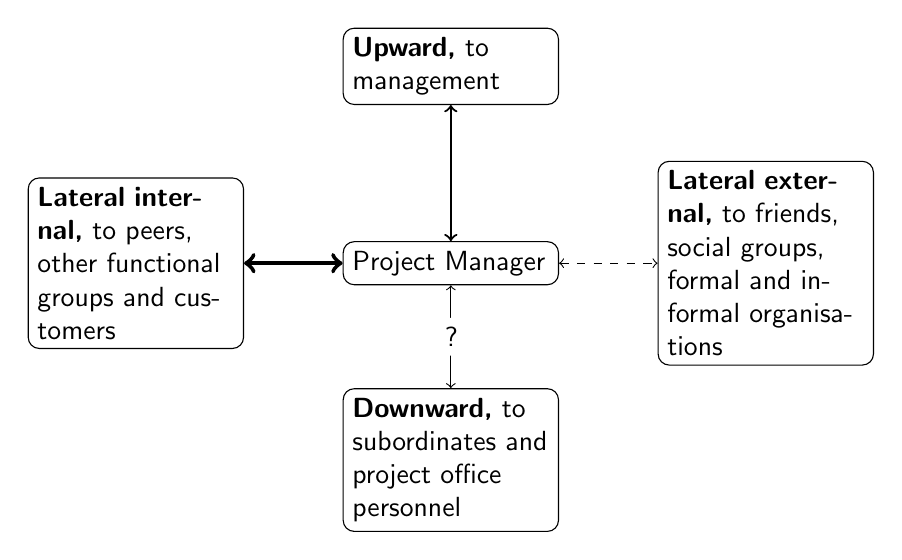
\begin{tikzpicture}
    \newcommand{\mybox}[1]{#1}
        \tikzset{every node/.style={
            draw, rounded corners,
            text width=2.5cm,
            font=\sffamily
            }}
        \node (pm) at (0,0) {\mybox{Project Manager}};
        \node (up) at (0,2.5) {\mybox{\textbf{Upward,} to management}};
        \node (down) at (0,-2.5) {\mybox{\textbf{Downward,} to subordinates and project office personnel}};
        \node (left) at (-4,0) {\mybox{\textbf{Lateral internal,} to peers, other functional groups and customers}};
        \node (right) at (4,0) {\mybox{\textbf{Lateral external,} to friends, social groups, formal and informal organisations}};  
        \draw[<->,thick] (pm) -- (up);
        \draw[<->] (pm) -- node[draw=none,text width=1ex,fill=white] {?} (down);
        \draw[<->,ultra thick] (pm) -- (left);
        \draw[<->,dashed] (pm) -- (right);
    \end{tikzpicture}
\end{document}
